\subsection{Head Mount} 
As described earlier in the section \ref{sec:nao:vision}, integrated hardwares of NAO Vision are not sufficient to provide precise three dimensional data to the complex algorithms to track human skeletal joints. Therefore, Asus Xtion PRO LIVE 3D camera is chosen to be used for this gesture recognition system. Section \ref{sec:sol:impl} shows the final architecture that proposes to mount Asus Xtion on the head of the robot. 

\begin{figure}	 	
	\begin{minipage}
		{.45 
			\textwidth} 
		\centering 
		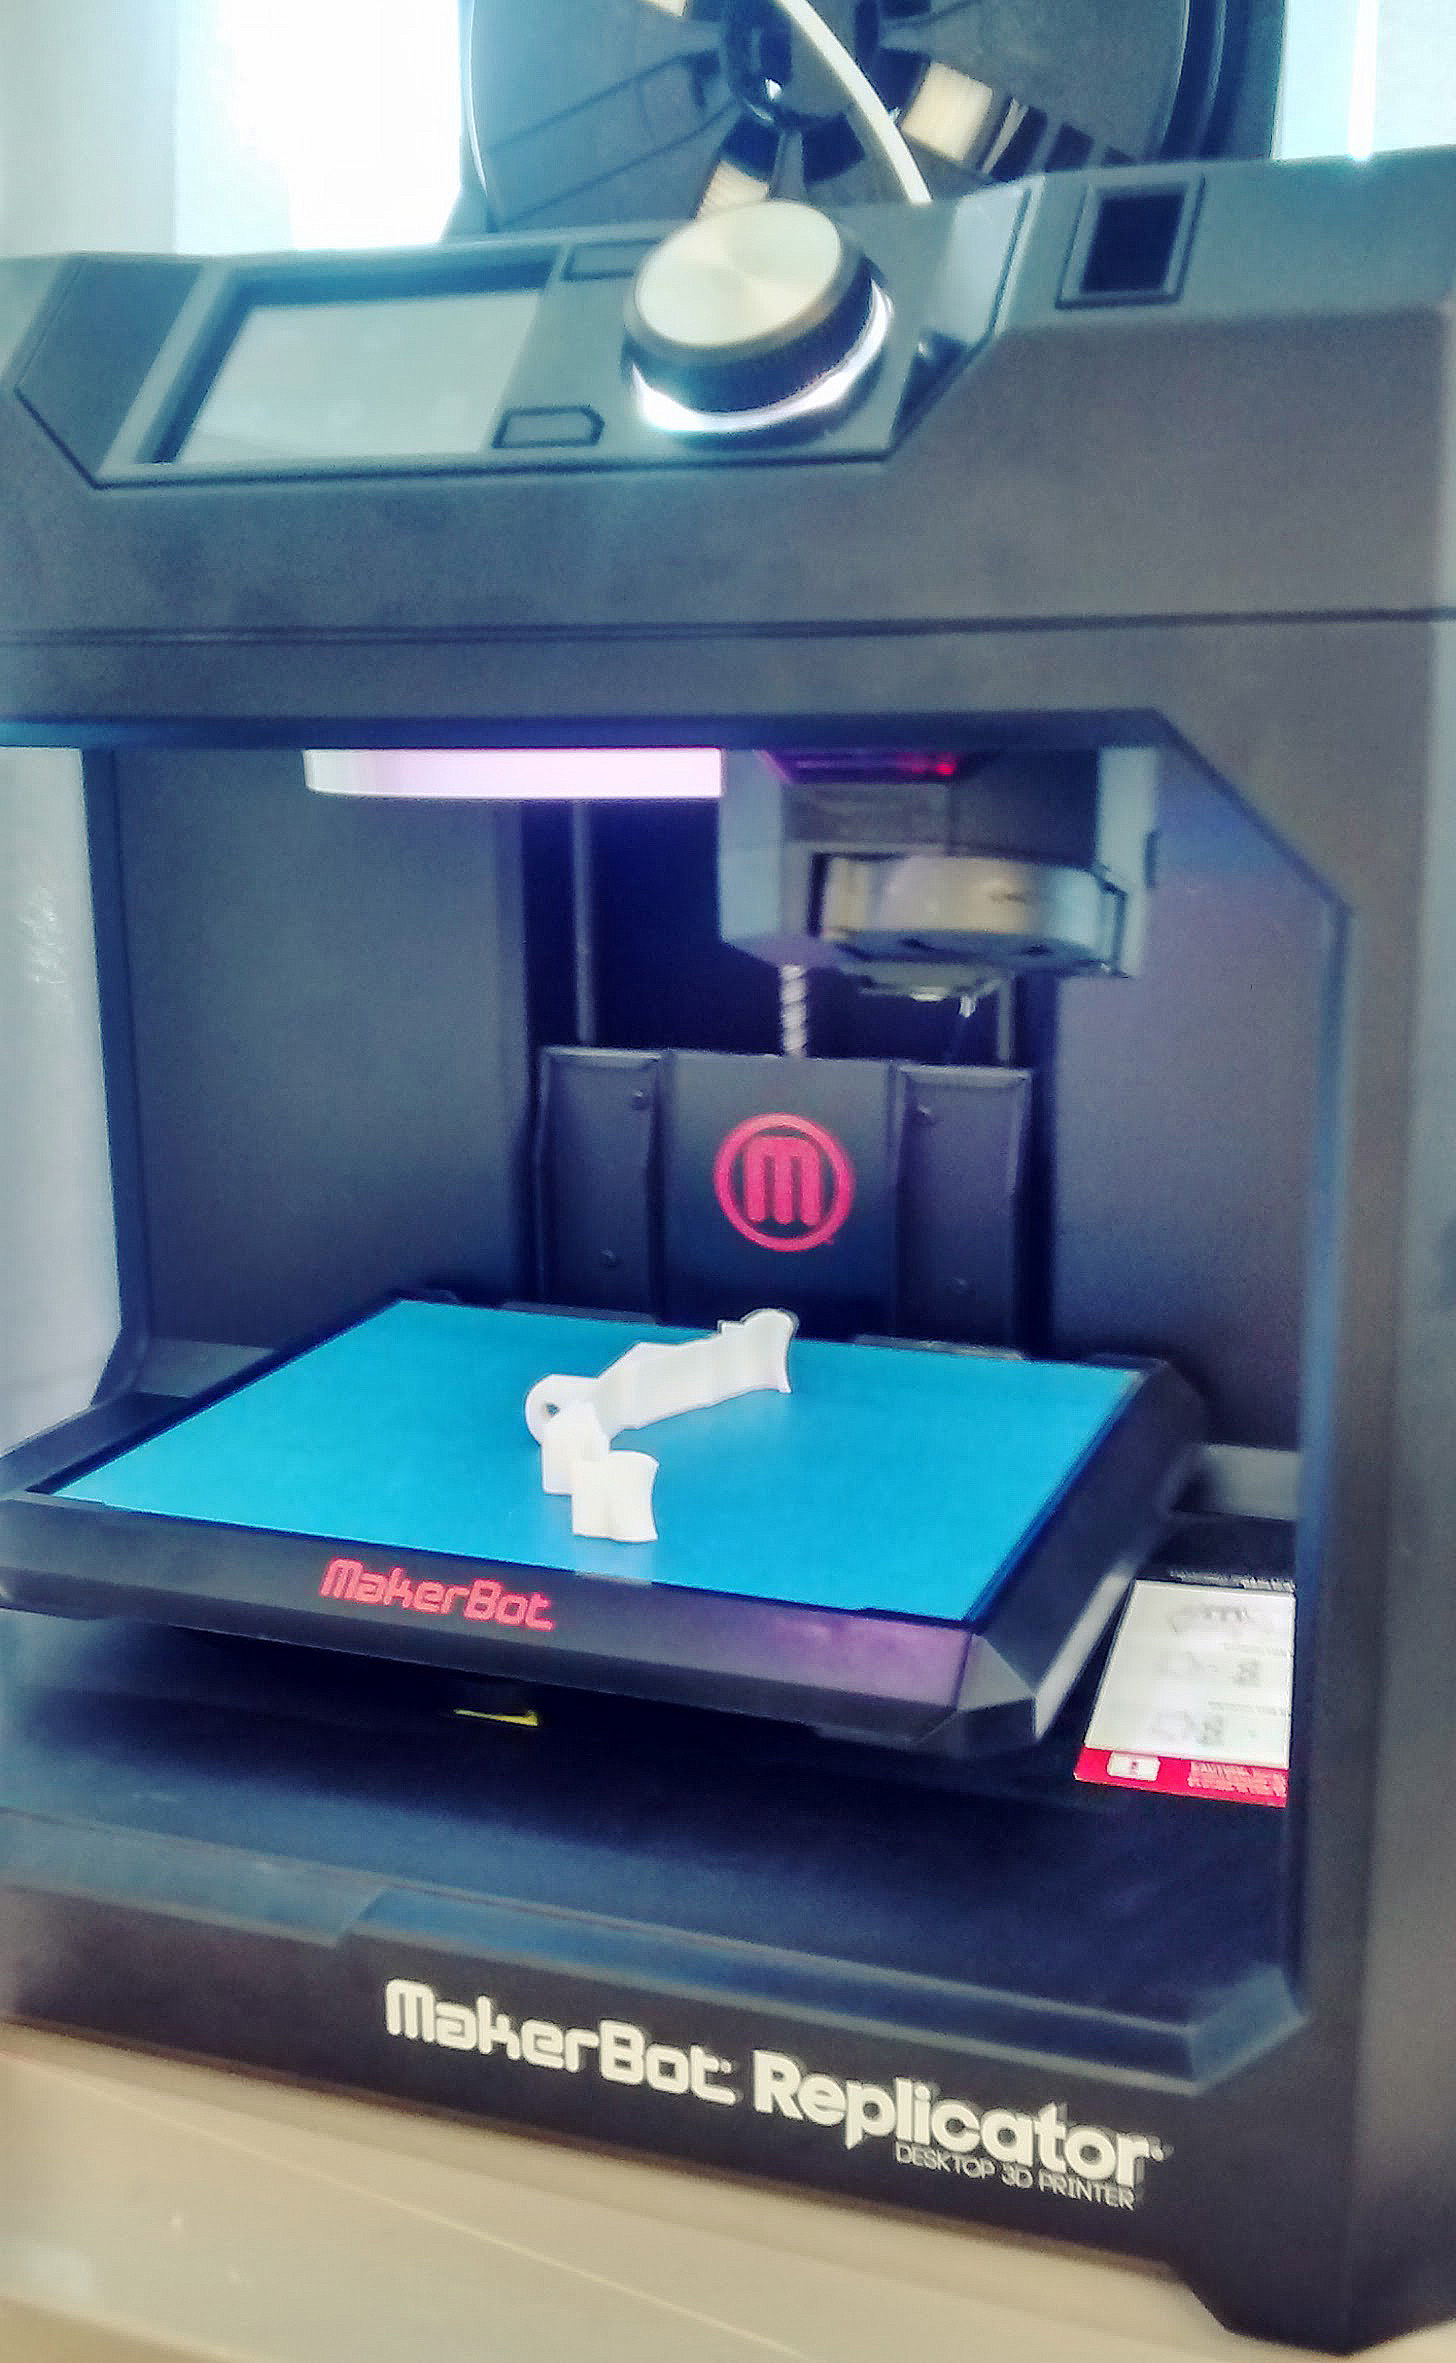
\includegraphics[height=60mm]{figures/content/xtion-mount-3d.jpg} \caption*{3D printing the mount} 
	\end{minipage}
	\begin{minipage}
		{.45 
			\textwidth}  
		\centering
		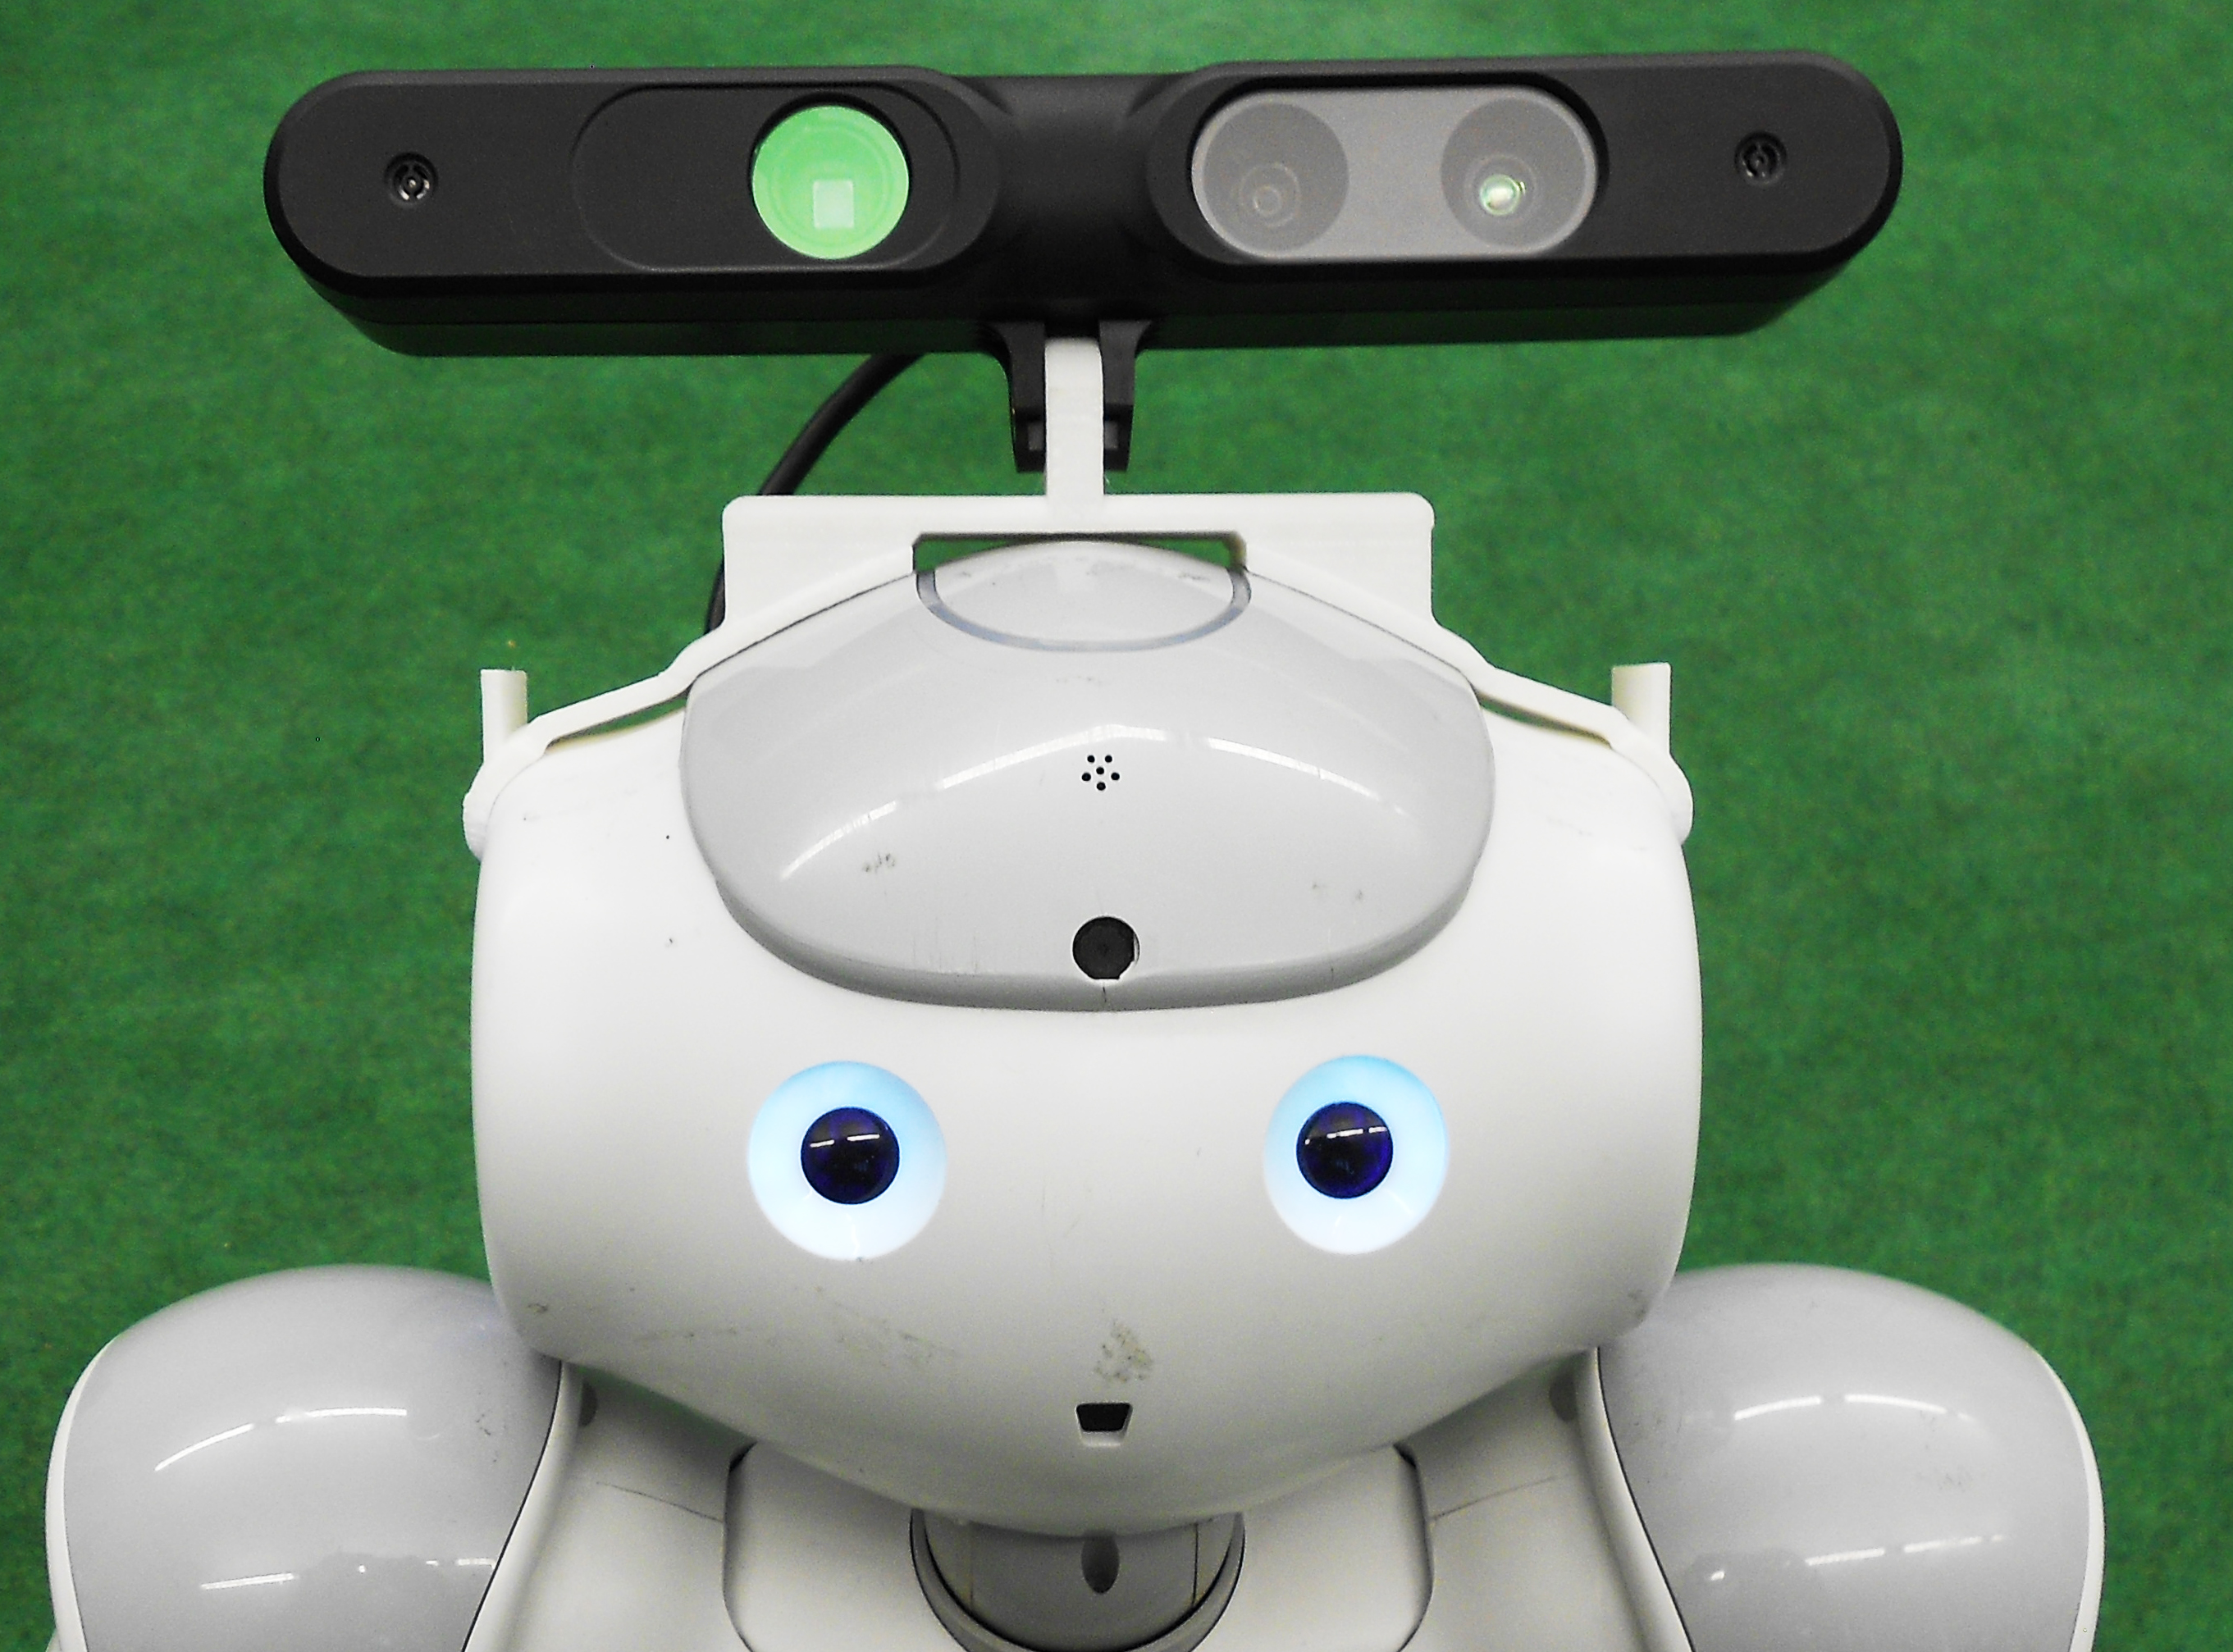
\includegraphics[height=60mm]{figures/content/xtion-mount.jpg} \caption*{Asus Xtion mounted on NAO}
	\end{minipage}
\end{figure}
\label{fg:xtion:mount}



\paragraph*{3D Printed NAO Xtion Mount} We have found a solution that was designed by emotion-robotics.com. Therefore, we have used their 3D model to print it using MakerBot Replicator 5th Generation 3D Printer as shown in the figure \ref{fg:xtion:mount}. The original base of Asus Xtion was removed and the camera was screwed with the 3D printed mount, and easily fixed on the head of the robot. 

